\section{Virtual Memory Management}
bla

\subsection{Aufbau}
bla

Abbildung \ref{fig:largePageTranslation} zeigt die Umwandlung einer vom ARM Prozessor erzeugten virtuellen Adresse in eine physikalische Speicheradresse. Die Umwandlung wird vollständig durch die Prozessor-Hardware durchgeführt.

\begin{figure}
	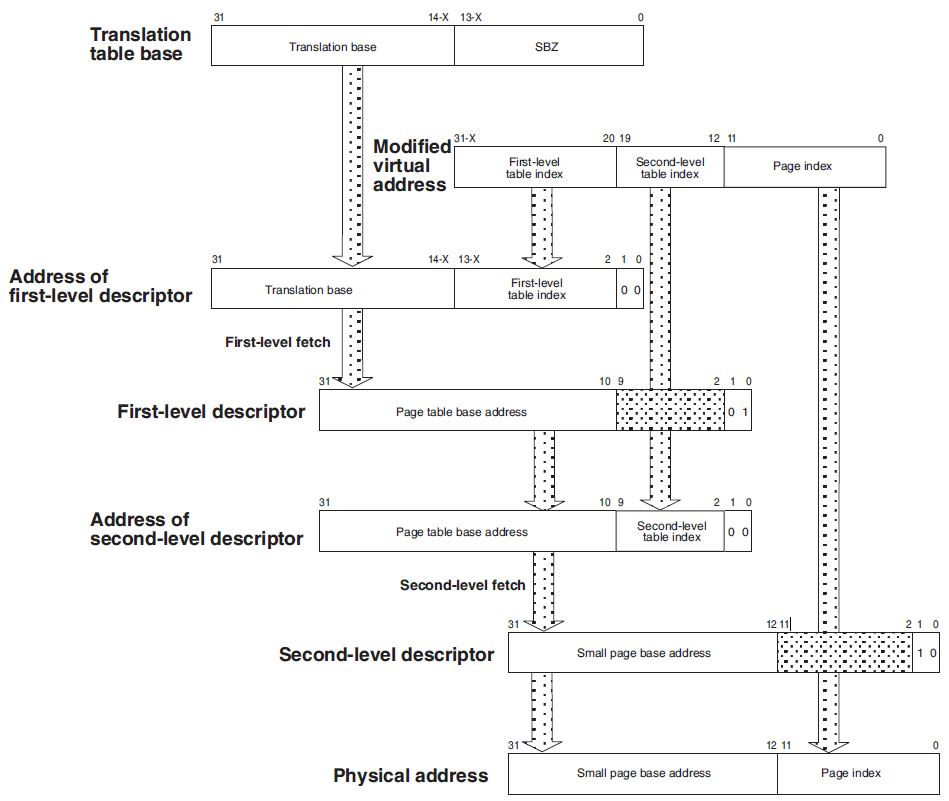
\includegraphics[scale=0.8]{figures/largePageTranslation}
	\caption{Umwandlung einer virtuellen Adresse durch zweistufiges Tabellensystem}
	\label{fig:largePageTranslation}
\end{figure}


\begin{figure}
	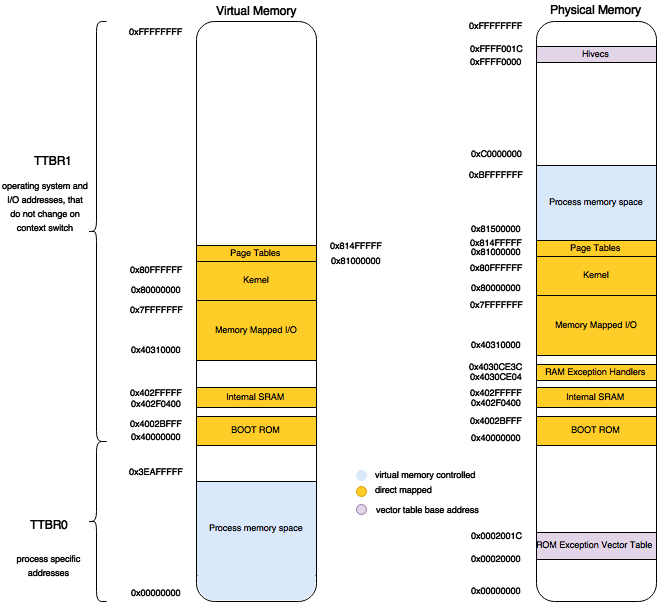
\includegraphics[scale=0.7]{figures/MemoryMap}
	\caption{Memory Map des Betriebssystems}
	\label{fig:MemoryMap}
\end{figure}


\begin{figure}
	\centering
	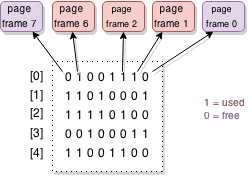
\includegraphics[scale=1]{figures/BitsMap}
	\caption{Beispiel einer Bitsmap zur Verwaltung der Page Frames}
	\label{fig:BitsMap}
\end{figure}

\pagebreak 